\section{Синтез комбинационной схемы}

\subsection{Постановка задачи}

На вход демультиплексора синхронно во времени с трехразрядным кодом адреса поступает информационный сигнал, 
который следует передать на один из 5-ти выходов, соответствующий коду адреса на входе демультиплексора. 
Задать в табличной форме функцию переходов и синтезировать 
комбинационную схему демультиплексора с одним информационными входом, 3-х разрядным кодом адреса и 5-ю выходами.

\subsection{Описание алгоритма синтеза комбинационной схемы}

Алгоритм синтеза комбинационной схемы состоит в следующем:

\begin{enumerate}
    \item Построить таблицу истинности устройства.

    \item Минимизировать функции выходных сигналов.

    \item Синтезировать комбинационную схему устройства.
    
    \item Конец алгоритма.
\end{enumerate}

\subsection{Построение таблицы истинности}

Построим таблицу истинности для демультиплексора с входным сигналом $x$, адресными - $a_1$, $a_2$, $a_3$ и выходными - 
$y_1$, $y_2$, $y_3$, $y_4$, $y_5$.

\begin{table}[h!]
    \caption{Таблица истинности демультиплексора}
    \begin{tabular}{| >{\centering}m{0.05\textwidth} 
                    | >{\centering}m{0.05\textwidth} 
                      >{\centering}m{0.05\textwidth} 
                      >{\centering}m{0.05\textwidth} 
                    | >{\centering}m{0.05\textwidth} 
                      >{\centering}m{0.05\textwidth} 
                      >{\centering}m{0.05\textwidth} 
                      >{\centering}m{0.05\textwidth} 
                      >{\centering\arraybackslash}m{0.05\textwidth}|} 
        \hline $x$ & $a_1$ & $a_2$ & $a_3$ & $y_1$ & $y_2$ & $y_3$ & $y_4$ & $y_5$ \\
        \hline  0  &   0   &   0   &   0   &   -   &   -   &   -   &   -   &   -   \\
        \hline  0  &   0   &   0   &   1   &   0   &   0   &   0   &   0   &   0   \\        
        \hline  0  &   0   &   1   &   0   &   0   &   0   &   0   &   0   &   0   \\
        \hline  0  &   0   &   1   &   1   &   0   &   0   &   0   &   0   &   0   \\
        \hline  0  &   1   &   0   &   0   &   0   &   0   &   0   &   0   &   0   \\       
        \hline  0  &   1   &   0   &   1   &   0   &   0   &   0   &   0   &   0   \\ 
        \hline  0  &   1   &   1   &   0   &   -   &   -   &   -   &   -   &   -   \\ 
        \hline  0  &   1   &   1   &   1   &   -   &   -   &   -   &   -   &   -   \\ 
        \hline  1  &   0   &   0   &   0   &   -   &   -   &   -   &   -   &   -   \\ 
        \hline  1  &   0   &   0   &   1   &   1   &   0   &   0   &   0   &   0   \\ 
        \hline  1  &   0   &   1   &   0   &   0   &   1   &   0   &   0   &   0   \\ 
        \hline  1  &   0   &   1   &   1   &   0   &   0   &   1   &   0   &   0   \\
        \hline  1  &   1   &   0   &   0   &   0   &   0   &   0   &   1   &   0   \\
        \hline  1  &   1   &   0   &   1   &   0   &   0   &   0   &   0   &   1   \\
        \hline  1  &   1   &   1   &   0   &   -   &   -   &   -   &   -   &   -   \\ 
        \hline  1  &   1   &   1   &   1   &   -   &   -   &   -   &   -   &   -   \\     
        \hline
    \end{tabular}
    \label{tab:task3:truth_table}
\end{table}

\subsection{Минимизация функций выходов}

На рисунке \ref{fig:task3:karnaugh} показаны карты Карно с наибольшими покрытиями для функций выходов:
а - $y_1$; б - $y_2$; в - $y_3$; г - $y_4$; д - $y_5$.

\vspace{1em}

\begin{figure}[ht]
    \centering
    \begin{tabular}{cccc}
        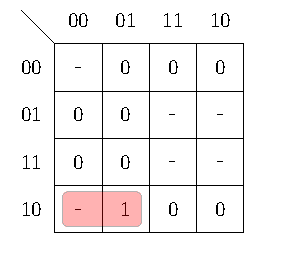
\includegraphics[width=0.3\textwidth]{S3IM1.pdf} &
        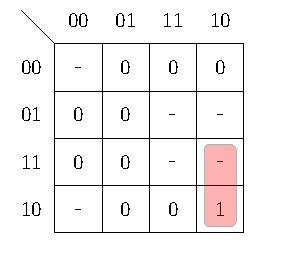
\includegraphics[width=0.3\textwidth]{S3IM2.pdf} &
        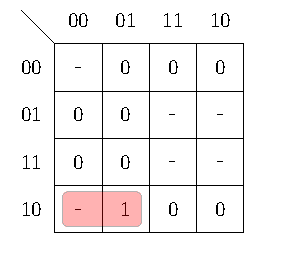
\includegraphics[width=0.3\textwidth]{S3IM1.pdf} \\
        a & б & в \\[1em]
    \end{tabular}
    %
    \begin{tabular}{cccc}
        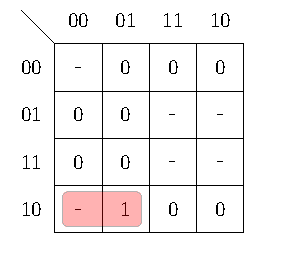
\includegraphics[width=0.3\textwidth]{S3IM1.pdf} &
        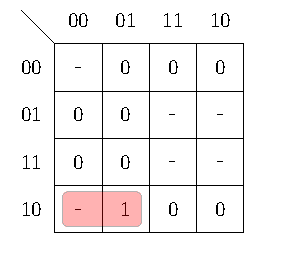
\includegraphics[width=0.3\textwidth]{S3IM1.pdf} \\
        г & д \\[1em]
    \end{tabular}

    \caption{Карты Карно для функций выходов $y_i$}
    \label{fig:task3:karnaugh}
\end{figure}

По наибольшим покрытиям минтермов получим минимальные формы для каждой функции $y_i$:

\begin{equation}
    y_1 = x \bar{a_1} \bar{a_2}
    \label{eq:task3:formula1}
\end{equation}

\begin{equation}
    y_2 = x a_2 \bar{a_3}
\end{equation}

\begin{equation}
    y_3 = x a_2 a_3
\end{equation}

\begin{equation}
    y_4 = x \bar{a_2} \bar{a_3}
\end{equation}

\begin{equation}
    y_5 = x a_1 a_3
    \label{eq:task3:formula5}
\end{equation}

\subsection{Синтез комбинационной схемы демультиплексора}

Синтезируем комбинационную схему демультиплексора
с одним информационным входом, трехразрядным адресныим входом
и пятью информационными выходами, заданными функциями (\ref{eq:task3:formula1}) - (\ref{eq:task3:formula5}).

\begin{figure}[ht]
    \centering
    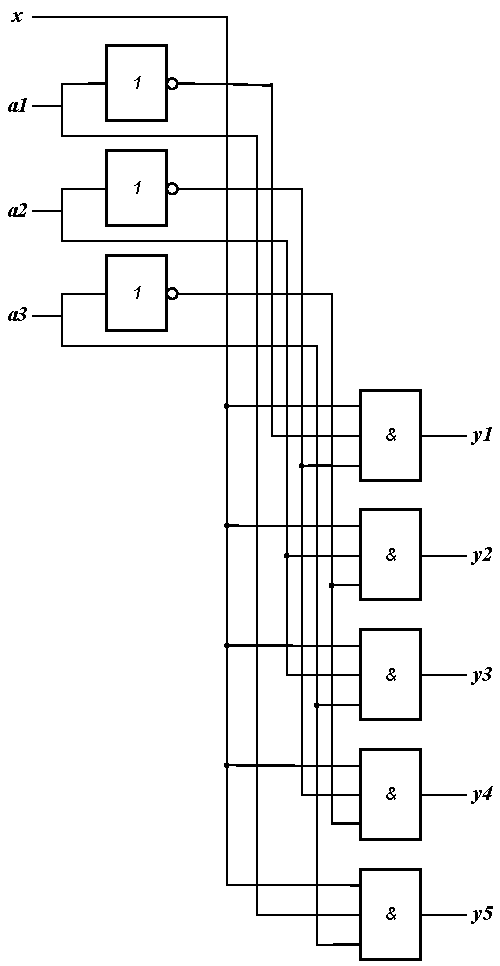
\includegraphics[scale=1]{S3IM6.pdf}  
    \caption{Структурная схема демультиплексора}
    \label{fig:task3:scheme}
\end{figure}